\section{Blockchain suffix proofs}
We now provide a concrete NIPoPoW construction which allows proving certain
predicates $Q$ of the chain $\chain$.
Among the predicates which are stable, in this section, we will limit ourselves to \textit{suffix sensitive} predicates.
%These predicates are easier to prove, but are not expressive enough for our applications. Nonetheless,
We extend the protocol to support more flexible predicates (such as transaction inclusion, as needed for our applications) in Section~\ref{sec:infix}.

\begin{definition}[Suffix sensitivity]
A chain predicate $Q$ is called $k$-\textnormal{suffix sensitive} if for all
chains $\chain, \chain'$ with $|\chain| \geq k$ and $|\chain'| \geq k$ such that
$\chain[-k:] = \chain'[-k:]$ we have that $Q(\chain) = Q(\chain')$.
\end{definition}

Notice that if a predicate $Q$ is suffix-sensitive, then then its value must be determined only by the $k$-suffix of the chain.

\noindent\textbf{Example.}
In general our applications will require predicates that are not suffix-sensitive. However, as an example, consider the predicate ``an Ethereum contract at address $C$ has been initialized with code $h$ at least $k$ blocks ago'' where $h$ does not invoke the \texttt{selfdestruct} opcode. This can be implemented in a suffix-sensitive way because in Ethereum, each block includes a merkle trie over all of the contract codes, which cannot be changed after initializtion. This predicate is thus also monotonic and $k$-stable.

\subsection{Construction}
We present a generic form of the verifier first and the prover afterwards. The
generic form of the verifier works with any practical suffix proof protocol.
Therefore, we describe the generic verifier first before we talk about the
specific instantiation of our protocol. The generic verifier is given access to
call a protocol-specific proof comparison operator $\leq_m$ that we define. We begin the
description of our protocol by first illustrating the generic verifier. Next, we
describe the prover specific to our protocol. Finally, we show the instantiation
of the $\leq_m$ operator, which plugs into the generic verifier to make a
concrete verifier for our protocol.

\noindent{\bf The generic verifier.}
The \textsf{Verify} function of our NIPoPoW construction  for suffix predicates
is described in
Algorithm~\ref{alg.nipopow-verifier}. The verifier algorithm is parameterized by
a chain predicate $Q$ and security parameters $k, m$; $k$
pertains to the amount of proof-of-work needed to bury a block so that it is
believed to remain stable (e.g., $k = 6$); $m$ is a security
parameter pertaining to the prefix of the proof, which connects the genesis
block to the $k$-sized suffix. The verifier receives several proofs by
different provers in a collection of proofs $\mathcal{P}$. Iterating over these
proofs, it extracts the best.

Each proof is a chain. For honest provers, these are subchains of the  adopted
chain. Proofs consist of two parts, $\pi$ and $\chi$; $\pi \chi$ must be a valid
chain; $\chi$ is the proof suffix; $\pi$ is the prefix. We require $|\chi| = k$.
For honest provers, $\chi$ is the last $k$ blocks of the adopted chain, while
$\pi$ consists of a selected subset of blocks from the rest of their chain
preceding $\chi$. The method of choice of this subset will become clear soon.

\import{./}{algorithms/alg.verifier-lite.tex}

The verifier compares the proofs provided to it by calling the $\geq_m$
operator. We will get to the operator's definition
shortly. Proofs are checked for validity before comparison by ensuring $|\chi| =
k$ and calling \textit{validChain} which checks if $\pi\chi$ is an anchored
blockchain.

The verifier loops through all candidate proofs $\pi$ and extracts the best one
$\tilde\pi$ using the $\geq_m$ operator for comparisons; $\tilde\chi$ is set to
be the suffix associated with the best known prefix. While $\tilde\chi$ is
needed for the final predicate evaluation, it is not used as part of any
comparison, as it has the same size $k$ for all proofs.

After the end of the for loop, the verifier will have determined the best proof
$(\tilde\pi, \tilde\chi)$. We will later prove that this proof will necessarily
belong to an honest prover with overwhelming probability. Since the proof has
been generated by an honest prover, it is associated with an underlying honestly
adopted chain $\chain$. The verifier then extracts the value of the predicate
$Q$ on the underlying chain.

\noindent
\textbf{The concrete prover.}
The NIPoPoW honest prover construction is shown in
Algorithm~\ref{alg.nipopow-prover}. The honest prover is supplied with an
honestly adopted chain $\chain$ and security parameters $m, k, \delta$ and
returns proof $\pi\chi$, which is a chain. The suffix $\chi$ is the last $k$
blocks of $\chain$. The prefix $\pi$ is constructed by selecting various blocks
from $\chain[:-k]$ and adding them to $\pi$, which consists of a number of
blocks for every level $\mu$. At the highest possible level at which at least
$m$ blocks exist, all these blocks are included. Then, inductively, for every
superchain of level $\mu$ that is included in the proof, the suffix of length
$m$ is taken. Then the underlying superchain of level $\mu - 1$ spanning the
same blocks as that suffix is also included, until level $0$ is reached. This
underlying superchain will have $2m$ blocks in expectation and always at least
$m$ blocks.

\import{./}{algorithms/alg.nipopow-prover.tex}

When we take a $\mu$-superchain and are interested in its last $m$ blocks, we
fill the same range of blocks with blocks from the superchain of level $\mu - 1$
below. All the $\mu$-superblocks which are within this $m$ blocks range
will also be $(\mu-1)$-superblocks and so we do not want to keep them
in the proof twice. Note that no check is necessary to
make sure the top-most level has at least $m$ blocks, even though the verifier
requires this. The reason is the following: Assume the blockchain has at least
$m$ blocks in total. Then, when a superchain of level $\mu$ has less than $m$
blocks in total, these blocks will all be necessarily included into the proof by
a lower-level superchain $\mu - i$ for some $i > 0$. Therefore, it does not hurt
to add them to $\pi$ earlier.

Figure~\ref{fig.nipopow} contains an example proof constructed for parameters
$m = k = 3$. The top superchain level which contains at least $m$ blocks is
level $\mu = 3$. For the $m$-sized suffix of that level, $5$ blocks of
superblock level $2$ are included for support spanning the same range. For the
last $3$ blocks of the level $2$ superchain, blocks of level $1$ are included
for support.

\begin{figure}[h]
    \caption{
    NIPoPoW prefix $\pi$ for $m = 3$ on a good chain.
    }
    \centering
    \iftwocolumn
        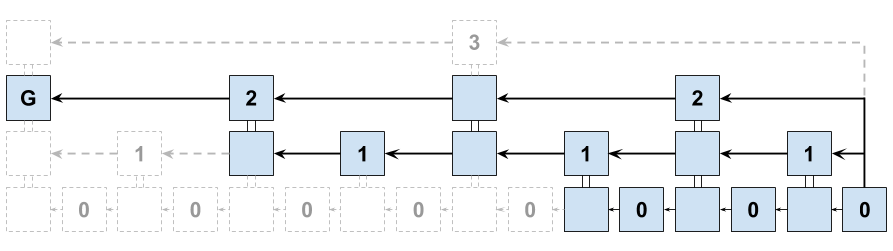
\includegraphics[width=\columnwidth,keepaspectratio]{figures/non-interactive-popow.png}
    \else
        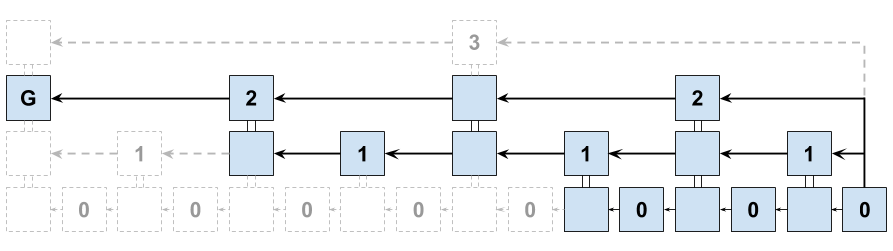
\includegraphics[width=0.7\columnwidth,keepaspectratio]{figures/non-interactive-popow.png}
    \fi
    \label{fig.nipopow}
\end{figure}

\noindent
\textbf{The concrete verifier.}
The $\geq_m$ operator which performs the
comparison of proofs is presented in Algorithm~\ref{alg.nipopow-maxchain}. It
takes proofs $\pi_A$ and $\pi_B$ and returns true if the first proof is winning,
or false if the second is winning. It first computes the LCA block $b$ between the
proofs. As parties $A$ and $B$ agree that the blockchain is the same up to block
$b$, arguments will then be taken for the diverging chains after $b$. The best
possible argument from each player's proof is extracted by calling the
$\text{best-arg}_m$ function.
% We call the
% willingness of the verifier to allow each prover to be evaluated based on their
% best argument the \textit{principle of charity}.
To find the best argument of a proof $\pi$ given $b$, $\text{best-arg}_m$
collects all the $\mu$ indices which point to superblock levels that contain
valid arguments after block $b$. Argument validity requires that there are at
least $m$ $\mu$-superblocks following block $b$, which is captured by the
comparison $|\pi\upchain^\mu\{b:\}| \geq m$. $0$ is always considered a valid
level, regardless of how many blocks are present there. These level indices are
collected into set $M$. For each of these levels, the score of their respective
argument is evaluated by weighting the number of blocks by the level as
$2^\mu|\pi\upchain^\mu\{b:\}|$. The highest possible score across all levels is
returned. Once the score of the best argument of both $A$ and $B$ is known, they
are directly compared and the winner returned.  An advantage is given to the first proof in case of a tie by using the $\geq$ operator favouring $A$.

\import{./}{algorithms/alg.nipopow-maxchain.tex}
